\chapter{Application Flow Monitoring}

\itodo{
- Cisco Application Visibility and Control\\
- \url{http://www.cisco.com/c/en/us/products/routers/avc-control.html}\\
- \url{http://www.cisco.com/c/dam/en/us/solutions/collateral/enterprise-networks/unified-wan-services/at\_a\_glance\_c45-649117.pdf}\\
}

\itodo{
- Network-Based Application Recognition (NBAR)\\
- \url{http://www.cisco.com/c/en/us/products/collateral/ios-nx-os-software/network-based-application-recognition-nbar/product\_bulletin\_c25-627831.html}
}

\section{Creating Application Flow}

\iinfo{Taken from: Application Flow Monitoring Challenges}

\itodo{TODO: vyporadat se s opakujicimi se hlavickami (HTTP), doplnit definici flow z predchozi kapitoly\\
- Flow expiration/termination vs app flow splitting}

The application flow monitoring is a complex process. Packets need to be received from the network, transported to computer memory (RAM), parsed, aggregated to flow records based on the parsed information, and exported to flow collectors for further processing. The process is depicted in Figure~\ref{fig:flow-exporter-schema}. This section describes the whole flow measurement process, points out where it is affected by the application processing and introduces some of the related challenges.

\begin{figure}[t!]
  \begin{center}
    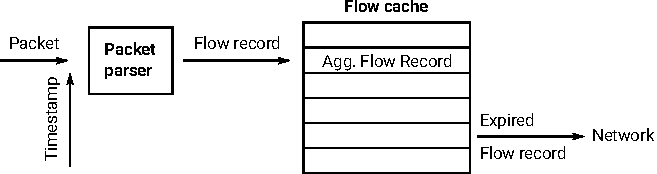
\includegraphics[width=\textwidth]{figures/flow-exporter-schema}
  \end{center}
  \caption{A Flow Exporter Schema}
  \label{fig:flow-exporter-schema}
\end{figure}

\subsection{Packet Reception}

The packet reception is unchanged for application flow monitoring unless the NIC processes the application layer. This scenario is discussed later in Hardware Accelerated Techniques section.


\subsection{Packet Parsing}

The basic task of the packet parsing is to extract connection attributes such as IP addresses, transport protocol, and ports to determine which flow the packet belongs to. Moreover, it obtains additional information of interest, especially from application protocols. The parser must be resilient to malformed packets and unknown protocols while supporting a wide range of existing network and application protocols.

Link, network, and transport headers of IP packets follow a strictly defined structure so that the network devices such as routers can process the packets swiftly. However, application layer protocols often rely on connections being established between compatible endpoints. For this reason, application protocol identification is a difficult task. A lot of attention has been dedicated to research of application identification in network traffic in the past, for example in the work of \citeauthor{Bujlow-2015-classification}~\cite{Bujlow-2015-classification}, however, not every approach is suitable for the flow monitoring scenario.

With increasing deployment of encryption for all kinds of communication, the task of application flow monitoring becomes more difficult. Without access to application payload, the amount of information that can be extracted from the traffic is diminished. However, there are statistical and machine learning methods that are able to recognize specific applications even in encrypted traffic with high accuracy. Moreover, useful information such as a version of encryption protocol, certificates, or supported cipher suites, can be extracted from encrypted traffic. This information can be used to identify malicious encrypted traffic. The possibilities of processing and analysis of encrypted traffic were surveyed by the authors of~\cite{Velan-2015-Survey}.

\subsection{Flow Aggregation}

Application protocol measurement may require flow record to be expired early. For example, when HTTP protocol supports pipelining, multiple requests and responses can be carried out over a single connection. When it is desirable to keep track of each request/response pair, existing flow record might be exported when a new request is encountered on the same connection. Therefore, application flow monitoring  also affects the number of generated flow records, which needs to be taken into consideration during further processing of the flow records.

\iimprove{TODO: keeping application data from expired flow records (long HTTP video streaming)}

Another impact of the application flow monitoring on the flow aggregation is the increased size of flow records. The information extracted from application protocols can be quite large in comparison to network and transport layers lengths. While the typical IPv4 header length is 20 bytes, typical TCP header length is 32 bytes, the HTTP URL can easily be several hundred bytes long. Therefore, the length of flow records of application flow monitoring is several times larger than without the application layer. There are two main negative impacts of such large flow records. Firstly, the flow cache might require much more RAM than standard flow monitoring flow cache. Secondly, even if the cache fits into RAM, it degrades the performance of the memory accesses because data locality is decreased and a CPU experiences more cache misses. For these reasons, it must be carefully considered which information is placed in each flow record and how it is encoded.

\subsection{Flow Export}

Several issues might be encountered with flow export when application flow monitoring is applied. First, due to the larger amount of exported data, the link to a flow collector might be congested. We have experienced this issue when application flow records from a 10G link were exported simultaneously to several collectors over old 100\,Mb/s management interface. The solution is either to simply upgrade to 1\,Gb/s management interface or, better, to reduce the number of targets of the export and distribute the flows as necessary through replicating proxy in the location of the collectors. The latter solution saves network bandwidth used for monitoring purposes and should be preferred if possible.

Another issue that might be encountered due to large flow record is that single record might be larger than MTU of the management network interface on the flow exporting device. In such a case UDP transport protocol, which is still widely used for flow export, cannot be used without fragmenting IP packets. The fragmentation might cause a performance problem for the flow collector which has to reassemble the packets. It also increases the probability of data loss as single lost fragment invalidates the whole message.

\section{Application Flow Benefits}

\itodo{Papers using application flows}

\section{Common Issues} % what is specific to application protocols, otherwise it should be at the end of previous chapter

% shortening of string values - add some indication of shortening or original length

\section{Conclusions}

\section{Relevant Publications}
\iunsure{Do it like rick and have it in the intro to each chapter?}